\vspace{-10pt}
\section{Appendix} \label{sec:append}

In the Appendix, the basic ideas of the proofs of Theorems~\ref{thm:alg-greedy}-\ref{thm:1dpa} are sketched.

\vspace{-10pt}
\subsection{Greedy Ratio Algorithm}

The basic idea of the proof of Theorem~\ref{thm:alg-greedy} is to compare the solution $X \cup \{j\}$ obtained by {\sc GRA} with the optimal solution. By the greedy order, each customer has a better or equal efficiency ratio than the corresponding optimum customer, when both the greedy and optimal solutions are considered according to the order $\frac{u_k}{|S_k|} \ge \frac{u_{k'}}{|S_{k'}|}$, when $k \le k'$. One can easily derive form this that the ratio of the total valuation of the set of customers in $X \cup \{j\}$ to the total valuation in any optimal set is bounded from below by the ratio of the sum of the absolutes of the demands in these two sets. It remains thus to bound  this ratio from below. This essentially amounts to relating the sum of the absolutes of a set vectors in $\CC$ to the absolute of the sum of these vectors, and can be shown by induction on the number of vectors. 

Fig.~\ref{fig:greedy} illustrates a tight extreme case when the optimum packs more power demands (in length) than that of {\sc GRA}. One can show by induction that the two  sides corresponding to $X^*$ (optimal sides) are equivalent (in the extreme case). Rescale all power demands such that each of the two optimal sides is equal to 1, then apply basic trigonometry 
$\sum_{k \in X \cup \{j\}}|S_k| = \sqrt{(1+\cos \theta)^2 + \sin^2 \theta} = \sqrt{2 + 2\cos \theta}$
Therefore, $\frac{\sum_{k \in X \cup \{j\} } |S_k|}{\sum_{k \in X^*} |S_k|} = \frac{\sqrt{2 + 2\cos \theta}}{2}=\sqrt{\frac{\cos \theta + 1}{2}}$
In this case, it follows that $u(X \cup \{j\}) \ge \sqrt{\frac{\cos \theta + 1}{2}} \cdot \OPT$. Finally, since the algorithm returns the maximum valuation of either $X$ or $\{j\}$, the solution objective is at least half of $X \cup \{j\}$.


\begin{figure}[!htb]
	\centering \vspace{-5pt}
		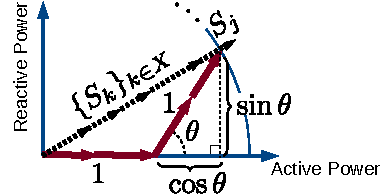
\includegraphics[scale=0.8]{fig/fig-greedy-brief.pdf} \vspace{-5pt}
\caption{The figure depicts an extreme case when the ratio  $\frac{\sum_{k \in X \cup \{j\}} | S_k|}{\sum_{k \in X^*} |S_k|}$ is minimal, where $X^*$ is an optimal solution. The dotted arrows represent solution $ X \cup \{j\}$ (which is infeasible), whereas the red solid arrows represent the optimal solution $X^*$. These two solutions constitute a triangle.}
	\label{fig:greedy}
\end{figure} 

\vspace{-20pt} 
\subsection{One-dimensional Projection Algorithm}

The basic idea of the proof of Theorem~\ref{thm:1dpa} is to divide the feasibility region into two parts: $\cD_1$ and $\cD_2$ (see Fig.~\ref{fig:proj}). There are three cases. (Case 1) If an optimal solution $X^*$ resides in $\cD_1$ (i.e., $\sum_{k \in X^*} S_k(t) \in \cD_1$), then it is equivalent to the classical knapsack problem with capacity $\frac{C}{\sqrt{2}}$, and ${\rm Alg}^{\rm kp}$ can find a close-to-optimal solution.  

(Case 2 and 3) On the other hand, if an optimal solution $X^*$ resides in $\cD_2$ (i.e., $\sum_{k \in X^*} S_k(t) \in \cD_2$), then one can show that it is either a singleton power demand with the maximum valuation, or a sum of power demands with at least half of valuation lies in $\D_1$ (which is equivalent to the classical knapsack problem with capacity $\frac{C}{\sqrt{2}}$). 

\begin{figure}[!htb]
\centering \vspace{-10pt}
\includegraphics[scale=0.60]{fig/{fig-0.5-proof2}.pdf} \vspace{-15pt}
\caption{The feasibility region is divided into $\cD_1$ and $\cD_2$. } 
\label{fig:proj}
\end{figure}